\documentclass[a0,landscape]{a0poster}
%\documentclass[a0,draft]{a0poster}
% With the word preview in the square bracket, your poster will be a4
% size, handy for previewing or submit to x4u queue for A0. 
% with preview removed, you get a file the right size for the HP
% large-format printer. This is a bit bigger than A0, the width is 
% exactly one imperial yard.

% This is so we can have multiple columns of text side-by-side
\usepackage[utf8]{inputenc}
\usepackage{graphicx}
\usepackage{multicol}
\usepackage{helvet}
\usepackage{sectsty}
%\allsectionsfont{\usefont{OT1}{phv}{bc}{n}\selectfont}
\allsectionsfont{\sffamily} \subsubsectionfont{\sffamily\large}
\columnsep=100pt 

% This is the thickness of the black line between the columns of text
\columnseprule=3pt

% this package gives you coloured text and various other simple
% graphics hacks. 
% Details in /usr/local/teTeX/texmf/doc/generic/pstricks/*
\usepackage{pstricks}

%\psset{unit=1cm}

\usepackage{times}
\usepackage{url}

% Define names for some colours 
\newcmykcolor{Inblue}{1.00 0.37 0.00 0.00}
\newcmykcolor{Inred}{0.00 1.00 0.63 0.00}
\newrgbcolor{Inmaroon}{0.4 0.0 0.4}
\newrgbcolor{darkblue}{0.0 0.0 0.5}

% Colour used for figure captions. Change to suit your own preference
\newrgbcolor{captcolor}{0.0 .5 0.0}

\begin{document}

% This is black magic to put a title at the top of the page.
% Thanks to Mark ``the magician'' Filipiak, although I have re-done a
% lot of the code here -- hopefully it is more robust.

% Make a box 0.55* width of poster for title and names
% If your title is long, replace 0.55 with something bigger and 
% make the box for the address smaller by the same amount.
\begin{minipage}[b]{0.75\linewidth} 
\veryHuge \bf 
\textsf{Rapid rule-based machine translation between Dutch and Afrikaans}
\\[1cm]
\huge \bf Pim Otte, Francis M. Tyers,\\
\huge \rm Mendelcollege, Universitat d'Alacant
\end{minipage}
% Make box 0.35 X width of poster for address  
\begin{minipage}[b]{0.25\linewidth} 
\Large 
Contact: 5666@mendelcollege.nl, ftyers@dlsi.ua.es \\

\end{minipage}
%% Make box 0.05*width of poster for EU Shield graphic
%\begin{minipage}[b]{0.05\linewidth}
%\includegraphics[width=10cm]{logo_ofis_liv.pdf}
%%\includegraphics{uitlogo}
%\end{minipage}
%\vspace{0.3cm}
%\hrule
%vspace{0.3cm}
%\begin{minipage}[b]{\linewidth} 
%\hrule
%{\small \url{http://www.ofis-bzh.org/bzh/ressources_linguistiques/index-troerofis.php}}
%\end{minipage}
%

% This is how many columns your poster will be broken into.
\begin{multicols}{4}

% This is the width your figures will be scaled to. Change this if you 
% change the number of columns.
\newlength{\figwidth}
\setlength{\figwidth}{20cm}

% Set to half of figwidth. Used for putting two figs side by side
\newlength{\fighalfwidth}
\setlength{\fighalfwidth}{10cm}

% Can't use the figure environment within multicolumns. Set up our own 
% counter for figures.
\newcounter{figscount}

\section{Introduction}

\noindent
{\bf Dutch} is a West-Germanic language spoken by nearly 23 million people, mostly from the 
Netherlands and Flanders. {\bf Afrikaans} is spoken by at least 5 million people, mainly in 
South-Africa, but also in Namibia. Afrikaans also belongs to the West-Germanic language family and originates from the language 
spoken by the the Dutch colonists of the Cape Colony. In 1925 Afrikaans replaced Dutch as
an official language in South-Africa, to be the joint official language together with English.
On this poster we will describe the development of {\small {\tt apertium-af-nl}}, a bi-directional Afrikaans 
and Dutch machine-translation system

\begin{center}
\begin{minipage}[b]{26cm}
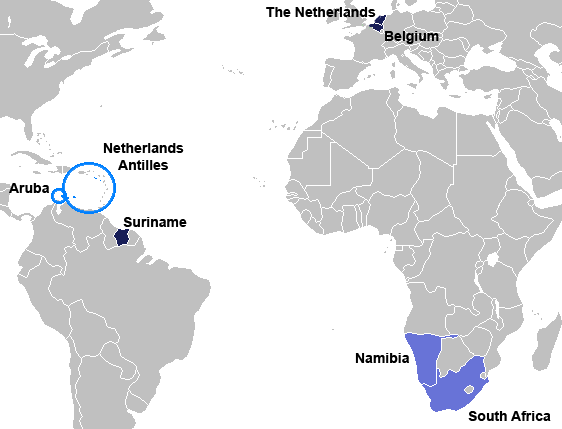
\includegraphics[width=260mm]{mapdutchworld.png}
\end{minipage}\\
\textbf{Figure 1:} Where Afrikaans or Dutch is spoken as official language.
\vspace{0.3cm}
\end{center}

%\vspace{0.5cm}

\section{Method}

\noindent
The system is based on {\bf Apertium} (\url{http://www.apertium.org/}), a free/open-source rule-based
machine translation platform. To create the language pair we used an existing resource and created 
several new ones. \\

\begin{center}
\begin{minipage}[b]{26cm}
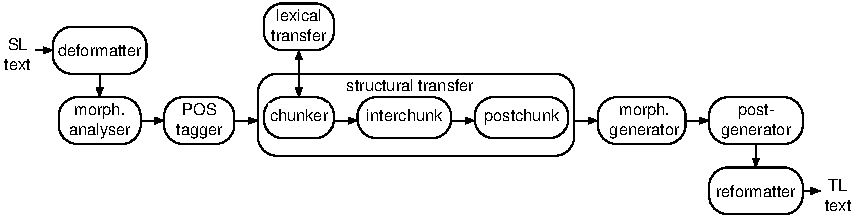
\includegraphics[width=260mm]{apertium2.pdf}
\end{minipage}\\
\textbf{Figure 2:} Modules of the Apertium translation system
\vspace{0.3cm}
\end{center}


\vspace{0.5cm}

\subsection{Existing resources}

\noindent
We reused the morphological transducer for Afrikaans, created during a currently dormant English-Afrikaans
Machine Translation project.\\

\subsection{Resources created}

\subsubsection{Dutch morphological transducer}
A new Dutch morphological transducer was created, because existing ones were unsuitable for several reasons:

\begin{itemize}
 \item Non-free licence
 \item Not bidirectional (only analysis, not generation)
 \item Tagset different from Afrikaans transducer
\end{itemize}

%\vspace{0.5cm}

\noindent
The open categories (nouns, verbs, adjectives, adverbs) for the Dutch 
morphological analyser were extracted semi-automatically from 
Wiktionary, (\url{http://www.wiktionary.org}), which has entries like in {\bf Figure 3}. The resulting analyser entries were all hand checked.
Closed categories were added by hand based on the grammar of Dutch of Shetter and Ham.
\vspace{0.5cm}

\begin{center}
\begin{minipage}[b]{26cm}
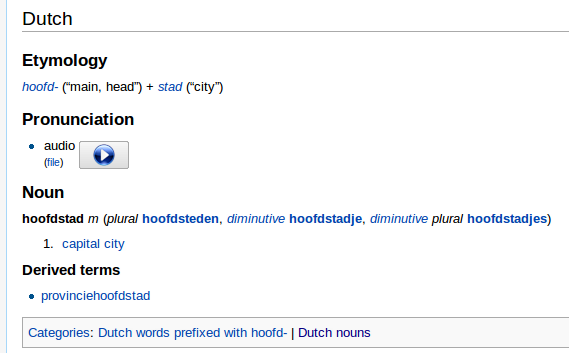
\includegraphics[width=260mm]{hoofdstad.png}
\end{minipage}\\
\textbf{Figure 3:} Example of Wiktionary entry: hoofdstad
\label{wikt1}
\vspace{0.3cm}
\end{center}


\vspace{0.5cm}

\subsubsection{Bilingual dictionary}

\noindent
The bilingual dictionary was developed by adding exact matches, extracting proper names
from Wikipedia, adding cognates, words which often have a small spelling difference and adding
some entries by hand, such as closed categories and frequently missing words.

\subsection{Transfer rules}

\subsubsection{Afrikaans to Dutch}
An example of an Afrikaans to Dutch transfer rule, which handles the negation scope marker, can be seen in
{\bf Figure 4}

\begin{center}
\begin{minipage}[b]{25cm}
\begin{scriptsize}
\begin{verbatim}
    <rule comment="REGLA: nie">
      <pattern>
        <pattern-item n="nie"/>
      </pattern>
      <action>
        <choose>
          <when>
            <test>
              <equal>
                <var n="seen_neg"/>
                <lit v="true"/>
              </equal>
            </test>
          </when>
          <otherwise>
            <out>
              <chunk name="nie">
                <tags>
                  <tag><lit-tag v="ADV"/></tag>
                </tags>
                <lu>
                  <clip pos="1" side="tl" part="lemh"/>
                  <clip pos="1" side="tl" part="a_adv"/>
                  <clip pos="1" side="tl" part="lemq"/>
                </lu>
              </chunk>
            </out>
          </otherwise>
        </choose>
        <let>
         <var n="seen_neg"/>
         <lit v="true"/>
        </let>
      </action>
    </rule>
\end{verbatim}
\end{scriptsize}
\end{minipage}\\
~\\
\textbf{Figure 4:} Transfer rule for handling negation.
\vspace{0.5cm}
\end{center}

\subsubsection{Compound words}
In both Afrikaans and Dutch words can combine very productively into compounds.
{\small {\tt apertium-af-nl}} can handle compounds that consist of one or more nouns, 
such as the one in {\bf Figure 5}. \\

\begin{center}
\begin{minipage}[b]{26cm}
\begin{small}
\begin{verbatim}
lugmag

^lug<n><sg><cmp>+mag<n><sg>$

^lucht<n><mf><sg><cmp>$^macht<n><mf><sg>$

luchtmacht
\end{verbatim}
\end{small}
\end{minipage}\\
\end{center}
~\\
\textbf{Figure 5:} Example of compound analysis and translation: lugmag (air force)



\subsubsection{Separable verbs}

\noindent
The system can handle separable verbs, which exist both in Afrikaans and Dutch, as
long as there are no other phrases between the separated parts.\\

\section{Evaluation}
\noindent
We evaluated the system in several ways: Naïve coverage, compound analysis, qualitative, quantitative and comparative

\subsection{Coverage}

\noindent
Naïve coverage was calculated over Wikipedia corpora.\\


\begin{minipage}[b]{25cm}
\begin{center}
  \begin{tabular}{|l|r|r|}
   \hline
   {\bf Corpus}           & {\bf Tokens}    & {\bf Coverage}\\
   \hline
   {\tt af} Wikipedia     & 2,926,943       & 82.1\% $\pm$ 0.8 \\
   \hline
   {\tt nl} Wikipedia     & 18,569,183      & 80.5\% $\pm$ 0.7 \\
   \hline
  \end{tabular}
    
 \end{center}
 \textbf{Table 1:} Na\"ive vocabulary coverage for the two morphological analysers.
\end{minipage}\\

\subsection{Compound words}
\noindent
To test the accuracy of the compound word analysis, we marked words as correctly segmented and/or 
correctly translated, this test was performed in the Afrikaans$\rightarrow$Dutch direction. \\

\begin{minipage}[b]{25cm}
  \begin{center}
  \begin{tabular}{|l|r|r|}
   \hline
   {\bf Corpus}    & {\bf Corr. Seg.}    & {\bf Corr. Trans.}\\
   \hline
   top-1,000       & 914                 &  776 \\ 
   \hline
   random-1,000    & 957                 &  801 \\ 
   \hline
  \end{tabular}
  \end{center}
  \textbf{Table 2:} Compound word accuracy in analysis and translation.
\end{minipage}\\

\subsection{Quantitative}  
\noindent
The translation quality was measured using word error rate (WER). For this we used sets
of 100 sentences from Wikipedia. The set C1 could not contain any unknown words, set C2 could. \\ 
\begin{minipage}[b]{25cm}
\begin{center}
  \begin{tabular}{|l|l|r|r|}
   \hline
   {\bf Dir.} & {\bf System}             & {\bf C1}          & {\bf C2} \\ 
   \hline
   {af-nl}  & {\small Apertium}  & 16.625 $\pm$ 1.465 & 23.405 $\pm$ 1.235 \\
            & {\small Google}  & {\bf 9.485 $\pm$ 1.115} & {\bf 10.575 $\pm$ 1.795} \\
   \hline
   {nl-af} & {\small Apertium }  & {\bf 15.435 $\pm$ 1.885}  & {\bf 21.72 $\pm$ 1.06} \\
           & {\small Google }  & 21.81 $\pm$ 1.72& 	25.71 $\pm$ 1.22	\\

   \hline
  \end{tabular}
    
    \label{table:quan}
  \end{center}
	\textbf{Table 3:} Accuracy for the test corpora for the two systems as measured by Word Error Rate 
        with 95\% confidence interval.
\end{minipage}\\

\subsection{Qualitative}
To discover which areas of the system could use the most improvement we reviewed the translation errors
in the Afrikaans$\rightarrow$Dutch direction and categorised them as in {\bf Table 4}. \\
\begin{minipage}[b]{25cm}
  \begin{center}
  \begin{tabular}{|l|c|r|r|}
     \hline
     {\bf Error type}    & {\bf Count} & {\bf \% of total} \\
     \hline
     Syntactic transfer   & 235         & 42.4 \\
     \hline
     ~~~- Verb concordance & 99          & 17.9 \\
     ~~~- Auxiliary verbs & 13          & 2.3 \\ 
     ~~~- Relative pronoun& 11          & 2.0 \\
     ~~~- Capitalisation  & 10          & 1.8 \\
     ~~~- Chunking error  & 9           & 1.6 \\
     ~~~- Other           & 93          & 16.8 \\
     \hline
     Unknown word         & 147         & 26.5 \\
     Disambiguation       & 106         & 19.1 \\
     Morphology           & 28          & 5.1 \\
     Polysemy             & 23          & 4.2 \\
     Multiword            & 6           & 1.1 \\
     Compounding          & 6           & 1.1 \\
     Separable verb       & 3           & 0.5 \\
     \hline
     Total                & 554         & 100 \\
     \hline
  \end{tabular}
    
  \end{center}  
     \textbf{Table 4:} Contribution to total error by type. Syntactic transfer errors are split into 
      further categories.
    
\end{minipage}\\

\subsection{Comparative}
Finally, we compared {\small {\tt apertium-af-nl}} with Google translate, using WER. The results 
are in {\bf Table 3}. {\bf Figure 6} is an example of an error, caused by wrong disambiguation. \\

\begin{itemize}
    \item[] Hier volg 'n lys van hoofstede. 
    \item[] Hier {\em volgen} een lijst van hoofdsteden. 
    \item[] Hier {\em volgt} een lijst van hoofdsteden.  
    \item[] `Here follows a list of capital cities.' 
\end{itemize}
\textbf{Figure 6:} Example of disambiguation error.

\section{Future work}
We have presented a bi-directional rule-based machine translation system between Dutch and Afrikaans.
The system gives promising results and offers improvement in the Dutch$\rightarrow$Afrikaans direction
over another public system, but does not offer improvement in quality in the other direction.

The three biggest issues in the system are:
\begin{itemize}
 \item Lack of dictionary coverage -- some common words are missing, such as kalender, rewolosie, binneland, silwer
 \item Poor morphological disambiguation -- work is needed to be able to, e.g. distinguish better between present and infinitive in Afrikaans
 \item Insufficient syntactic transfer -- separable constructions need more support, amongst which separable verbs and auxiliary verbs with participles.
\end{itemize}

\section*{Acknowledgements}
Development of this system was partially supported by the Google Code-in,
a contest to introduce pre-university students to contributing to open-source
software. This work has also received the support of the Spanish Ministry of Science and Innovation through project TIN2009-14009-C02-01.


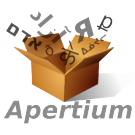
\includegraphics{apertium.png}





\end{multicols}
\end{document}

